\documentclass{standalone}

\usepackage{tikz}

\begin{document}

\setlength{\unitlength}{1in}

\begin{picture}(7.92, 6)
  \sffamily
  \put(-0.3, 0.2){\scalebox{1.4}{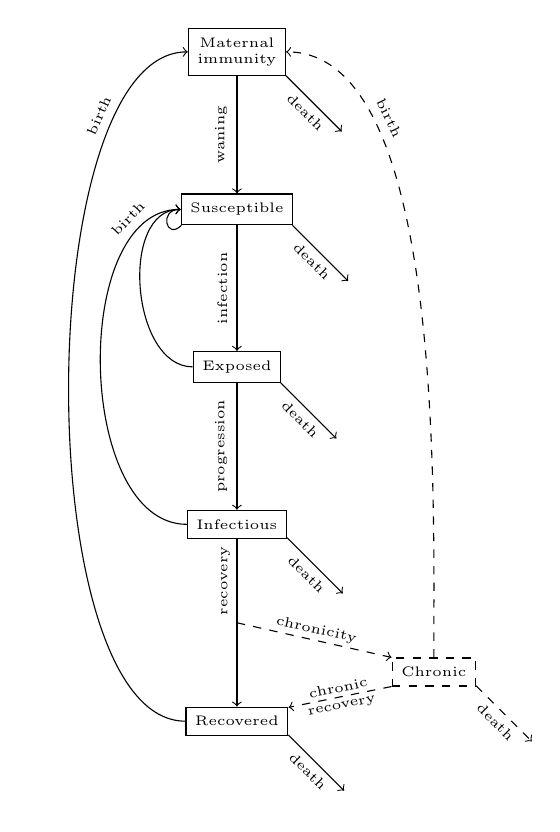
\begin{tikzpicture}[compartment/.style={rectangle, draw},
                    font=\fontsize{5pt}{6}\selectfont]
  % Compartments.
  \node at (0, 8.5) [compartment, align=center, name=MaternalImmunity] {Maternal\\immunity};
  \node at (0, 6.5) [compartment, name=Susceptible] {Susceptible};
  \node at (0, 4.5) [compartment, name=Exposed] {Exposed};
  \node at (0, 2.5) [compartment, name=Infectious] {Infectious};
  \node at (0, 0) [compartment, name=Recovered] {Recovered};
  \node at (2.5, 0.625) [compartment, dashed, name=Chronic] {Chronic};

  % Location for branch from Infectious to Chronic and Recovered.
  \coordinate (recovery) at (0, 1.25);

  % Infection-related processes.
  \draw [->] (MaternalImmunity)
             to node [rotate=90, above] {waning}
             (Susceptible);
  \draw [->] (Susceptible)
             to node [rotate=90, above] {infection}
             (Exposed);
  \draw [->] (Exposed)
             to node [rotate=90, above] {progression}
             (Infectious);
  \draw [  ] (Infectious)
             to node [rotate=90, above, yshift=-1pt] {recovery}
             (recovery);
  \draw [->, dashed] (recovery)
             to node [sloped, above, yshift=-2pt] {chronicity}
             (Chronic.161);
  \draw [->] (recovery)
             to node [] {}
             (Recovered.90);
  \draw [->, dashed] (Chronic.199)
             to node [sloped, align=center] {chronic\\recovery}
             (Recovered.15);
  % \draw [->] (Recovered.195)
  %            to [out=180, in=180] node [left, align=center] {immunity\\waning}
  %            (Susceptible.180);

  % Births
  \draw [->] (Susceptible.196)
             to [out=225, in=180, looseness=3.5] node [] {}
             (Susceptible.180);
  \draw [->] (Exposed.180)
             to [out=180, in=180] node [] {}
             (Susceptible.180);
  \draw [->] (Infectious.180)
             to [out=180, in=180, looseness=0.9] node [sloped, above, pos=0.85] {birth}
             (Susceptible.180);
  \draw [->] (Recovered.180)
             to [out=180, in=180, looseness=0.6] node [sloped, above, pos=0.8] {birth}
             (MaternalImmunity.180);
  \draw [->, dashed] (Chronic.90)
             to [out=90, in=0, looseness=0.65] node [sloped, above, pos=0.75] {birth}
             (MaternalImmunity.0);

  % Deaths
  \draw [->] (MaternalImmunity.334)
             to node [sloped, below, yshift=1pt] {death}
             +(315: 1);
  \draw [->] (Susceptible.344)
             to node [sloped, below, yshift=1pt] {death}
             +(315: 1);
  \draw [->] (Exposed.340)
             to node [sloped, below, yshift=1pt] {death}
             +(315: 1);
  \draw [->] (Infectious.345)
             to node [sloped, below, yshift=1pt] {death}
             +(315: 1);
  \draw [->] (Recovered.345)
             to node [sloped, below, yshift=1pt] {death}
             +(315: 1);
  \draw [->, dashed] (Chronic.342)
             to node [sloped, below, yshift=1pt] {death}
             +(315: 1);
\end{tikzpicture}

%%% Local Variables:
%%% mode: latex
%%% TeX-master: "diagram_standalone"
%%% End:
}}
  \put(3.3, 0){\includegraphics{figure_3_no_diagram}}
  % Separate panels in multi-part figures should be labelled with 8
  % pt bold, upright (not italic) a, b, c...
  \bfseries \footnotesize
  \put(-0.05, 5.9){(a)}
  \put(3.75, 5.9){(b)}
  \put(5.83, 5.9){(c)}
\end{picture}

\end{document}
